\documentclass[11pt, oneside]{article}   	% use "amsart" instead of "article" for AMSLaTeX format
\usepackage[margin=0.7in]{geometry}                		% See geometry.pdf to learn the layout options. There are lots.
\geometry{letterpaper}                   		% ... or a4paper or a5paper or ... 
%\geometry{landscape}                		% Activate for rotated page geometry
%\usepackage[parfill]{parskip}    		% Activate to begin paragraphs with an empty line rather than an indent
\usepackage{graphicx}				% Use pdf, png, jpg, or eps§ with pdflatex; use eps in DVI mode
								% TeX will automatically convert eps --> pdf in pdflatex		
\usepackage{amssymb}
\usepackage{amsmath}
\usepackage{amsfonts}
\usepackage{listings}
\usepackage{dsfont}
\usepackage{wasysym}

\newcommand{\Var}{\mathrm{Var}}


\title{A Simplified Model for Optimal Assembly Orificing in an SFR through Convex Optimization}
\author{Chris Keckler}
%\date{}							% Activate to display a given date or no date

\begin{document}
\maketitle

Due to the combination of radially and azimuthally varying material compositions and flux profile within a reactor core, each assembly will generate a different amount of heat during reactor operation.
Certain assemblies may generate much more power than others, for instance assemblies with large amounts of fissile material in high flux zones, or regions in which the flux is locally thermalized.
Others, such as blanket or control assemblies, may generate orders of magnitude less heat due to the fact that nearly all of their power comes from gamma heating.
The variation in assembly power generation is partly reflected in the radial peaking factor of a core, which gives the peak to average power radially across the core. 
Radial peaking factors for SFRs depend on the shuffling/batching strategy used for the reactor.
For standard batch-style SFRs where assemblies are not shuffled, peaking factors can be brought down by utilizing a checkerboard-style loading pattern or a heterogeneous core with internal blanket assemblies. 
For B\&B style SFRs of the standing-wave-type, the radial peaking factor is largely dependent on the radial shuffling pattern, but tends to be higher than that in a standard SFR design due to the physics of breeding.
Regardless, it is clear that the power generated in each assembly, and the corresponding amount of coolant required for each assembly, may vary drastically across the core.

The amount of coolant flowing through each assembly in an SFR is determined by a physical orifice placed at the bottom of each fuel assembly, which can be different from assembly to assembly.
Because SFR assemblies are canned and only communicate pressure between assemblies at the inlet and outlet plenums, the pressure drop over each assembly is the same.
The orifice creates a large, localized pressure drop which reduces the driving force for coolant flow, limiting the velocity and corresponding mass flow rate of coolant through the assembly.
Typically a limited number of orifice "zones" are desired so that (1) manufacturing complexity can be reduced and (2) flexibility exists with where a particular assembly can be placed in the core without violating thermal constraints.
Therefore, the core designer typically will group assemblies of similar powers together and make their orifices the same, giving the same flow rate to a group of assemblies.
This will result in a varying outlet temperature from each assembly within an orifice group, so it is important to effectively choose which assemblies are placed in a particular group so as to obtain acceptable temperatures.

The strategy for determining assembly orifice zones is different from reactor to reactor.
For metallic-fueled SFRs, often the goal is to minimize the peak inner-cladding temperature at the EOC, as this is when thermal conductivity has degraded the most and fuel-cladding eutectic reactions are the most likely to take place.
In an oxide core, eutectic reactions are not an issue, and instead peak fuel temperature at EOC is minimized due to large uncertainty in bulk fuel properties after irradiation.
Other reactors, such as a B\%B core, may be more restricted by other issues such as large power variations within a given assembly over the cycle length which could lead to overcooling and undercooling at various points in the cycle, penalizing plant thermodynamics.

However, underlying all of these different goals is the desire to have a relatively flat outlet temperature profile, and therefore a flat power-to-flow ratio profile.
This could clearly be achieved by simply orificing each assembly individually, however as outlined above, this is undesirable for a variety of reasons.
Therefore, a primary task of the reactor designer is to determine which assemblies will be grouped together and how much flow to give to that group.
This problem is subject to a number of constraints, but in general has many solutions, which makes the process of determining orificing zones somewhat arbitrary.
To date, this problem has been tackled through many algorithms and on many different levels of fidelity, ranging from subchannel analysis to simple energy balances.
All of these may give acceptable answers, but it is difficult to say in the end which orificing strategy provides the optimal solution, if indeed there is one.
The purpose of this paper is to define the problem of determining orifice zones as one of convex optimization so that optimal solutions may be found.
This is done using simplified models and generalized constraints, and implemented into MATLAB using the convex optimization solver CVX.
This work aims to develop a tool which can be used for very quick preliminary orificing determination.
This tool can then be used in tradeoff studies on the number of orifice zones for a reactor design and to provide a high-quality, detailed initial guess for the orificing to be further refined and validated through the use of higher fidelity software, such as subchannel codes.

%%%%%%%%%%%%%%%%%%%%%%%%%%%%%%%%%%%%%%%%%%%%%%%%%%%%%%%%%%%%%%%%%%%%%%%
\section{Problem Formulation}


%%%%%%%%%%%%%%%%%%%%%%%%%%%%%%%%%%%%%%%%%%%%%%%%%%%%%%%%%%%%%%%%%%%%%%%
\subsection{Basic Formulation}

Because the basic desire is to minimize the variation in outlet temperatures, a reasonable starting point for the formulation of this problem is to minimize the variation in outlet temperatures across all assemblies.
This could trivially be done for any particular outlet temperature, so to constrain the problem, it is imposed that the perfectly mixed outlet coolant temperature is equal to some temperature specified by the plant thermodynamics, $\bar{T}_{out}$.
Additionally, any meaningful results must have all flow rates positive.
The formulation therefore begins as:

\begin{align}
\min_{\dot{m}} \Var [T_{out}] \quad : \quad & \frac{\sum_i T_{out,i} \dot{m}_i}{\sum_i \dot{m}_i} = \bar{T}_{out} \\
& \dot{m} \geq 0 \nonumber
\end{align}

where $\dot{m} \in R^q_+$ is the vector of mass flow rates over all assemblies, $T_{out} \in R^q_+$ is the vector of outlet temperatures in each assembly, and $\bar{T}_{out}$ is a constant perfectly-mixed outlet coolant temperature.

The objective function can be expanded by simply using an energy balance over each individual assembly, which is accurate in steady-state as long as the heat capacity of the coolant does not appreciably change over the height of the assembly.
It is noted that for sodium, the value of $c_p$ is a weak function of temperature in this temperature range (see for instance, \cite{SAS_sodiumCorrelations}).
Rearranging the first constraint with this expansion allows for a more clear picture of the formulation.

\begin{align} 
\min_{\dot{m}} \Var [\frac{\dot{Q}}{\dot{m}c_p} + T_{in}] \quad : \quad & \sum_i \dot{m}_i = \frac{\sum_i \alpha_i}{\bar{T}_{out}-T_{in}}  \label{eq:nonConvexVersion} \\ 
& \dot{m} \geq 0 \nonumber
\end{align}

where $\dot{Q} \in R^q_+$ is the vector of powers generated in each assembly and $\alpha \in R^q_+$ is simply $\frac{\dot{Q}}{c_p}$, element-wise.
In the objective function, the division is also meant as element-wise.
Simple evaluation of this formulation reveals that it cannot be made to be convex due to $\dot{m}$ being in the denominator and numerator of the objective and constraints, respectively.
However, because the variance in the outlet temperature is what should be minimized, rather than simply the absolute temperatures, we can simply use the change in temperature across the assembly, as all assemblies have the same inlet temperature.
Furthermore, using similar reasoning, minimizing the variance in $\Delta T$ is the same as minimizing the variance in $\frac{1}{\Delta T}$.
This simple yet powerful insight allows for Equation \ref{eq:nonConvexVersion} to be reformulated in a convex manner as Equation \ref{eq:convexVersion}.

\begin{align}
\min_{\dot{m}} \Var [\frac{\dot{m}}{\alpha}] \quad : \quad & \sum_i \dot{m}_i = \frac{\sum_i \alpha_i}{\bar{T}_{out}-T_{in}} \label{eq:convexVersion} \\
& \dot{m} \geq 0 \nonumber
\end{align}

%%%%%%%%%%%%%%%%%%%%%%%%%%%%%%%%%%%%%%%%%%%%%%%%%%%%%%%%%%%%%%%%%%%%%%%
\subsection{Additional Constraints}

Although the formulation in Equation \ref{eq:convexVersion} is a good starting point, it does not account for a variety of practical constraints that would be placed upon a realistic design.
Chiefly among these practicalities is that the current formulation does not limit the number of orifice zones.
Because of this, actually the formulation in Equation \ref{eq:convexVersion} is not very useful, as it will simply return a unique flow rate for each assembly that makes the assembly reach the desired outlet temperture.
Therefore the formulation presented above has a unique solution which is trivially obtained. 

In order to limit the design space and make the calculation more realistic, a number of additional constraints are identified as

\begin{enumerate}
\item \label{list:maxTemp}coolant outlet temperatures should remain below boiling or some other specified lower temperature 
\item \label{list:dP} coolant pressure drop over the core should remain within the capability of the primary pump
\item \label{list:v_max} coolant flow velocity should remain below a particular threshold in order to avoid flow-induced vibrations
\item \label{list:adjacent} difference between outlet temperatures of adjacent assemblies should remain below a given threshold to avoid thermal striping
\end{enumerate}

Item \ref{list:maxTemp} can be taken care of easily by limiting the temperature increase over every assembly to remain below a given value, as each assembly has the same inlet temperature.
Equation \ref{eq:maxTemp} shows this constraint, inverted to keep the formulation convex.

\begin{align}
\frac{\dot{m}_i}{\alpha_i} \geq \frac{1}{\Delta T_{max}} \quad \forall i \label{eq:maxTemp}
\end{align}

Item \ref{list:dP} is somewhat more complicated to take into account, simply because the pressure drop across the assembly height is a complicated function of flow rates, temperatures, and geometry.
However, using a simplified model, we can roughly account for the pressure drop over the assembly as long as the geometry and general flow characteristics are known.
For a standard SFR assembly, most of the loss coefficients are reasonably well quantified and available in \cite{Waltar}.
Additionally, flow friction losses can be accounted for by using a proper friction loss coefficient, calculated, for instance, with the Novendstern model assuming an estimate for the Reynolds number.
This constraint takes the form of Equation \ref{eq:dP}, where $L$, $D$, $h$, and $A_f$ are known from the geometry, $K$ is supplied by the user based upon assembly design (and does not include assembly orifice losses), $f$ is from an appropriate friction loss model, and $\rho$ is supplied by the user based upon the average coolant temperature.
Although not linear, this constraint is clearly convex in $\dot{m}$.

\begin{align}
K \frac{\dot{m}_i^2}{2 \rho A_f^2} + f \frac{L}{D} \frac{\dot{m}_i^2}{2 \rho A_f^2} + \rho g h \leq \Delta P_{max}  \quad \forall i \label{eq:dP}
\end{align}

Item \ref{list:v_max} is trivially accounted for by breaking the mass flow rate into its constituent parts as shown in Equation \ref{eq:v_max}.

\begin{align}
\frac{\dot{m}_i}{\rho A_f} \leq v_{max} \quad \forall i \label{eq:v_max}
\end{align}

Finally, item \ref{list:adjacent} is more difficult to implement. 
Ideally, the constraint should be of the form Equation \ref{eq:adjacent1}, where $\nu$ is a user-supplied tolerance and the '$\perp$' symbol is used to mean adjacent assemblies.

\begin{align}
| T_{out,n} - T_{out,p} | \leq \nu \quad n \perp p \label{eq:adjacent1}
\end{align}

This can then be split up into two constraints to remove the absolute value, and $T_{out}$ can be replaced by $\Delta T$ to form

\begin{align}
\frac{\alpha_n}{\dot{m}_n} - \frac{\alpha_p}{\dot{m}_p} & \leq \nu \quad n \perp p \\
-(\frac{\alpha_n}{\dot{m}_n} - \frac{\alpha_p}{\dot{m}_p}) & \leq \nu \quad n \perp p \nonumber
\end{align}

However, the Hessians of these constraints are indefinite, meaning they are not convex. 
An alternative approximation that gives the same results is to restrict the temperature increase in each adjacent assembly to a specified percentage of the temperature increase within the current assembly.
This is shown in Equation \ref{eq:adjacent}, where $\eta$ is the prescribed percentage that neighboring assemblies must remain within.

\begin{align}
\frac{\dot{m}_n}{\alpha_n} \geq \frac{1}{1+\eta} \frac{\dot{m}_p}{\alpha_p} \quad n \perp p \label{eq:adjacent} \\
\frac{\dot{m}_n}{\alpha_n} \leq \frac{1}{1-\eta} \frac{\dot{m}_p}{\alpha_p} \quad n \perp p \nonumber
\end{align}

Although this does not limit the difference between assemblies to a specified strict amount, as does the constraint in \ref{eq:adjacent1}, this constraint is effective at keeping the outlet temperatures of adjacent assemblies close to each other, and, importantly, it is convex.
The user may target a specific threshold, of say 50 C difference between adjacent assemblies, by dividing the target value by the expected average temperature increase over the assemblies, which should be roughly $\bar{T}_{out} - T_{in}$. 
Results may then be tuned by adjusting $\eta$ according to the calculated results.

%%%%%%%%%%%%%%%%%%%%%%%%%%%%%%%%%%%%%%%%%%%%%%%%%%%%%%%%%%%%%%%%%%%%%%%
\subsection{Assembly Grouping}

One of the most important parts of the orificing strategy is choosing which assemblies to group together based upon their power production.
To do this as part of the optimization calculation presents a formidable challenge, as this introduces discrete quantities and makes the optimization problem of the mixed-integer combinatorial type.
Coping with this would require a much more robust solver than is used for the current optimization procedure, so instead a simplified approach is taken.

During the initialization phase of the optimization procedure, assemblies are first grouped together based upon their power using logarithmically spaced bins between the minimum and maximum powers.
Logarithmically spaced bins are used as opposed to linearly spaced bins due to the fact that assembly powers may vary over multiple orders of magnitude, from multiple megawatts for central driver assemblies to only tens of kilowatts in shield assemblies. 
Using linearly spaced bins has a tendency to group together shield and blanket assemblies that are relatively low in power compared to drivers, but still vary by many multiples within the same bin.
This leads to difficulty in obtaining a proper flow rate to cool such drastically differing power levels within the lowest orifice zone.
A more realistic approach is to then use logarithmically spaced bins, where the power-to-flow ratio within each assembly of a given orifice zone remains more constant.
A depiction of the two different binning approaches is shown in Figure \ref{fig:binning}, with all of the assemblies between a set of horizontal lines being in the same orifice zone.
It is clear that the logarithmically spaced binning produces a much more logical distribution for orificing.

\begin{figure}[h!]
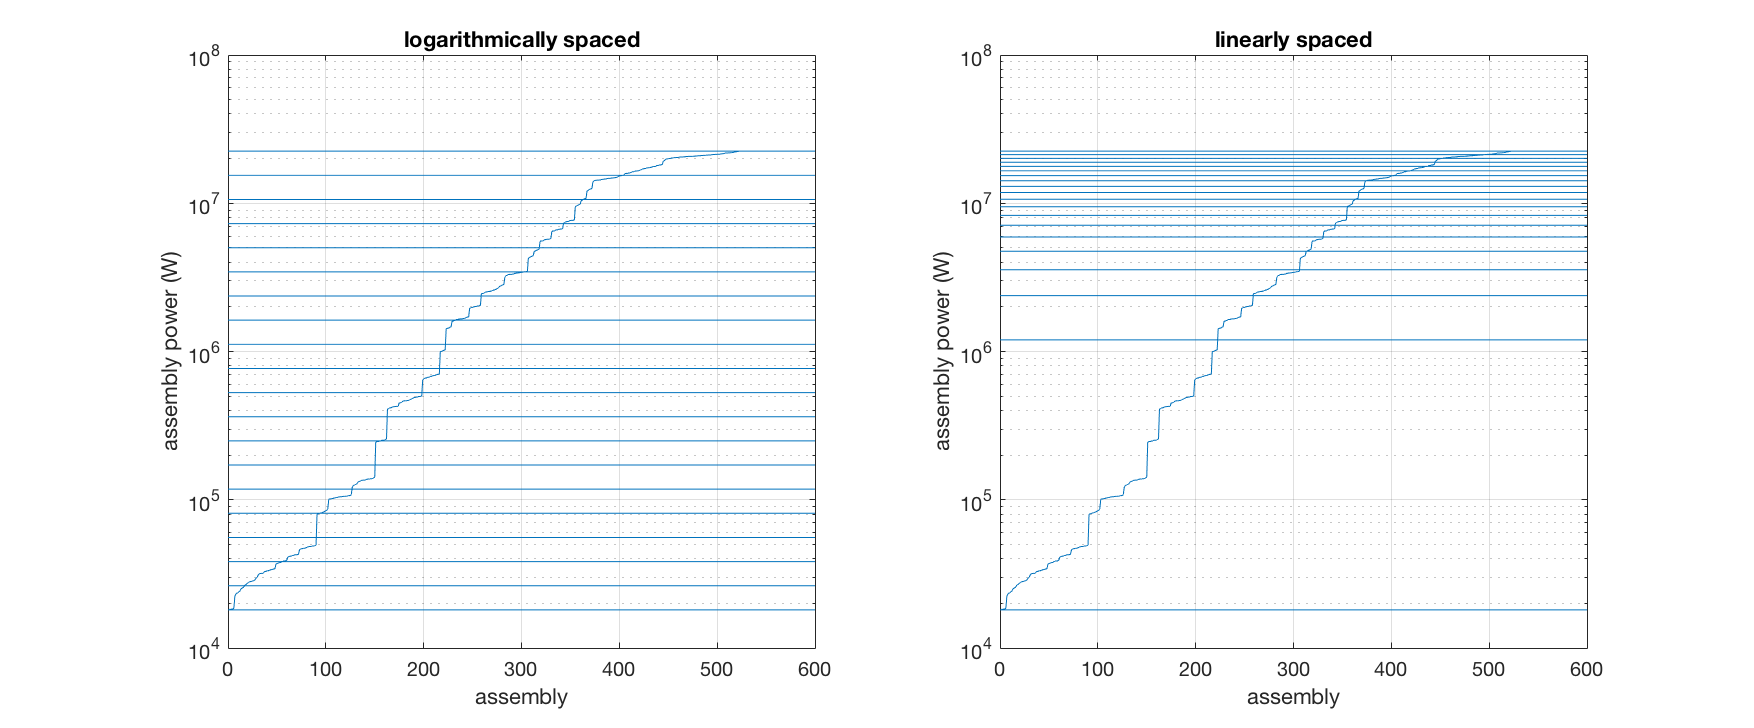
\includegraphics[width=18cm]{binning}
\centering
\caption{Orifice group boundaries determined using logarithmically and linearly spaced bins for a large core B\&B reactor with 20 orifice zones.}
\label{fig:binning}
\end{figure}

%%%%%%%%%%%%%%%%%%%%%%%%%%%%%%%%%%%%%%%%%%%%%%%%%%%%%%%%%%%%%%%%%%%%%%%
\subsection{Final Formulation}

\begin{align*}
\min_{\dot{m}} \Var [\dot{\frac{m}{\alpha}}] \quad : \quad & \dot{m} \geq 0 \\
& v_{max} \geq \frac{\dot{m}_i}{\rho A_f} \quad \forall i \\
& \dot{m}_j = \dot{m}_l \quad  j,l \in \chi_m \quad m = 1, \dots, k \\
& \frac{\dot{m}_i}{\alpha_i} \geq \frac{1}{\Delta T_{max}} \quad \forall i \\
& \sum_{i} \dot{m}_i \geq \frac{\sum_{i} \alpha_i}{\bar{T}_{out} + \gamma - T_{in}} \\
& \sum_{i} \dot{m}_i \leq \frac{\sum_{i} \alpha_i}{\bar{T}_{out} - \gamma - T_{in}} \\
& \frac{\dot{m}_n}{\alpha_n} \geq \frac{1}{1+\eta} \frac{\dot{m}_p}{\alpha_p} \quad n \perp p \\
& \frac{\dot{m}_n}{\alpha_n} \leq \frac{1}{1-\eta} \frac{\dot{m}_p}{\alpha_p} \quad n \perp p \\
& \Delta P_{max} \geq K \frac{\dot{m}_i^2}{2 \rho A_f^2} + f \frac{L}{D} \frac{\dot{m}_i^2}{2 \rho A_f^2} + \rho g h \quad \forall i \\
\end{align*}

%%%%%%%%%%%%%%%%%%%%%%%%%%%%%%%%%%%%%%%%%%%%%%%%%%%%%%%%%%%%%%%%%%%%%%%
\section{Code Use}

meant for use with Serpent hex lattice tallies

must include photon heating for blankets/control assemblies

friction losses use the Novendstern model

%%%%%%%%%%%%%%%%%%%%%%%%%%%%%%%%%%%%%%%%%%%%%%%%%%%%%%%%%%%%%%%%%%%%%%%
\begin{thebibliography}{9}


\end{thebibliography}

\end{document}